%%%%%%%%%%%%%%%%%%%%%%%%%%%%%%%%%%%%%%%%%%%%%%%%%%%%%%%%%%%%%%
% ECE 445 SENIOR DESIGN TEMPLATE
%%%%%%%%%%%%%%%%%%%%%%%%%%%%%%%%%%%%%%%%%%%%%%%%%%%%%%%%%%%%%
\documentclass[letterpaper,10pt]{article}

%%%%%%%%%%%%%%%%%%%%%%%%%%%%%%%%%%%%%%%%%%%%%%%%%%%%%%%%%%%%%
% The preamble starts here.
% You can add other packages that you want to use by using
% \usepackage command in the preamble.
% However, DO NOT change the settings that are already placed
% below unless you really know what you are doing.
%%%%%%%%%%%%%%%%%%%%%%%%%%%%%%%%%%%%%%%%%%%%%%%%%%%%%%%%%%%%%

% some commonly used packages\
\usepackage{siunitx}
\usepackage{graphicx}
\usepackage{color,soul}
\usepackage{amsmath}
\usepackage{amsthm}
\usepackage{amsfonts}
\usepackage{setspace}
\usepackage{longtable}
\usepackage{url}
\usepackage{pdfpages}
\usepackage{float}
\usepackage{rotating}
\usepackage{caption}
\usepackage{booktabs}  % professional-looking tables
\usepackage{multicol} %used for getting multicolumn without page-break
\usepackage{multirow}	% multi-row tables
\usepackage{array}		% define column format of a table
\usepackage[colorlinks=true,linkcolor=black,citecolor=black]{hyperref}
\usepackage[top=1.1in, bottom=1.1in, left=1.1in, right=1.1in]{geometry}% set the page margins to 1 inch
\usepackage{amsmath}
\usepackage{algorithm}
\usepackage[noend]{algpseudocode}
\usepackage{subfig}


% use the fancyhdr package to maintain the format of the page numbers,
% which is useful when the text color is changed
\usepackage{fancyhdr}
\fancyhf{}
\renewcommand{\headrulewidth}{1pt}
\renewcommand{\footrulewidth}{0pt}
\fancyfoot[C]{\textcolor{black}{\thepage}}
\fancyhead[L]{
\includegraphics[width=2cm]{University-of-Illinois-logo.jpg}}
\fancyhead[R]{\small{Infantry I.F.F. Final Report - Meyers \& Prince}}

% paralist provides extended list environments
\usepackage{paralist}
\setlength{\plitemsep}{0pt}

% define the color for section and subsection titles
\usepackage{xcolor}
\definecolor{titlecolor}{RGB}{31,73,125}
\definecolor{subtitlecolor}{RGB}{79,129,189}

% change the style of the section and subsection titles
\usepackage{titlesec}
\titleformat{\section}{\color{titlecolor}\Large\bf}{\color{titlecolor}\thesection}{0.8em}{}
\titleformat{\subsection}{\color{subtitlecolor}\large\bf}{\color{subtitlecolor}\thesubsection}{1em}{}
\titleformat{\subsubsection}{\color{subtitlecolor}\normalsize\bf}{\color{subtitlecolor}\thesubsubsection}{1.2em}{}
\titlespacing{\section}{0pt}{0em}{0em}
\titlespacing{\subsection}{6pt}{0em}{0em}
\titlespacing{\subsubsection}{12pt}{0em}{0em}



% change the style of the table of contents
\usepackage{titletoc}
\titlecontents{section}[1.5em]{}{\contentslabel{1.5em}}{\hspace*{-1.5em}}{\titlerule*[0.5pc]{.}\contentspage}
\titlecontents{subsection}[3em]{}{\contentslabel{2.1em}}{\hspace*{-2.1em}}{\titlerule*[0.5pc]{.}\contentspage}
\titlecontents{subsubsection}[5.1em]{}{\contentslabel{2.7em}}{\hspace*{-2.7em}}{\titlerule*[0.5pc]{.}\contentspage}

% command for centering texts in a fixed width table cell
\newcommand{\centpcol}{\leftskip\fill \rightskip\fill}

% command for setting the style of the appendix titles
\newcommand{\setappenstyle}{
	\titleformat{\section}{\color{titlecolor}\Large\bf}{\color{titlecolor}Appendix \Alph{section}}{0.8em}{}
	\titlecontents{section}[0em]{}{Appendix \thecontentslabel \hspace{1em}}{}{\titlerule*[0.5pc]{.}\contentspage}
}

\makeatletter
\newcommand{\skipitems}[1]{%
	\addtocounter{\@enumctr}{#1}%
}

% define the style of the title of the paper
\newcommand{\thetitle}[1]{\title{\begin{huge}{\bf #1}\end{huge} \color{subtitlecolor}\rule[25pt]{\textwidth}{1pt}}}

% define the style of the author
\newcommand{\theauthor}[3]{
	\author{\vspace{.4in}\\
	\textcolor{black}{By}\\
	#1
	\vspace{1in}\\
	\textcolor{black}{ECE 445 Final Report -} #2\\
	\textcolor{black}{TA:} #3
	\vspace{1in}}
}

% define the style of figure's caption
\newcommand{\figcap}[1]{
	\captionsetup{format=plain,font={small,color=subtitlecolor,singlespacing},margin={0pt,0pt}}
	\caption{\textcolor{subtitlecolor}{#1}}
	\vspace{-5pt}
}

% define the style of table's caption
\newcommand{\tablecap}[1]{
	\captionsetup{format=plain,font={bf,normalsize,singlespacing,color=black},margin={0pt,0pt}}
	\caption{\textcolor{black}{#1}}
	\vspace{-5pt}
}


\newcommand{\buildtoc}{
	\clearpage
	\singlespacing
	\tableofcontents
	\onehalfspacing
}

% set indentations and the space between paragraghs
\setlength{\parindent}{0pt}
\setlength{\parskip}{8pt}

\setcounter{secnumdepth}{4}

\titleformat{\paragraph}
{\normalfont\small\bfseries\color{subtitlecolor}}{\theparagraph}{1em}{}
\titlespacing*{\paragraph}
{18pt}{3.25ex plus 1ex minus .2ex}{1.5ex plus .2ex}

%%%%%%%%%%%%%%%%%%%%%%%%%%%%%%%%%%%%%%%%%%%%%%%%%%%%%%%%%%%%%
% PREAMBLE ENDS HERE, DOCUMENT STARTS BELOW
%%%%%%%%%%%%%%%%%%%%%%%%%%%%%%%%%%%%%%%%%%%%%%%%%%%%%%%%%%%%%

\begin{document}

% don't change these
\pagestyle{empty}
\doublespacing

% put the title of your project here. DO NOT include the brackets.
\thetitle{{I.F.F. (Identification Friend or Foe) System}}

% put your names here. seperate by \\. DO NOT include the brackets.
\theauthor{
	{Eric Meyers (emeyer7)}\\
	{Noah Prince (nprince2)}\\
}
{ % put the semester info here. DO NOT include the brackets.
	{Spring 2016}
}
{ % put your TA's name here. DO NOT include the brackets.
	{Brady Salz}
}

% put the date and project number here. DO NOT include the brackets.
\date{
{May 4th, 2016}\\
Project No. 11
\clearpage
}

% don't change these
\maketitle
\pagestyle{fancy}
\begin{spacing}{1.15}


% build the table of contents. 
\color{black}
\pagenumbering{gobble}
\section*{Abstract}
This project serves as a method for infantry units to identify friendly vs enemy combatants in the heat of battle. Quick and reliable friendly identification will reduce the number of friendly fire or misfire accidents in combat. A single LED indicator lights up identifying the target as a ``friendly." This could be extended to change the color of red-dot sites to green, similar to a reticle in a video game. 
\buildtoc
\pagenumbering{gobble}
\clearpage
\setcounter{page}{1}
\pagenumbering{arabic}

%SECTION - Introduction
\section{Introduction}
The purpose of this project is to create a system that quickly and accurately identifies friendly targets among military personnel on foot. Similar systems exist for aircraft, however not many exist for infantry.

The idea is to develop a two-way communication system so that when a soldier aims their weapon in the direction of a friendly target, they will receive notification through a light emitting diode (LED) that the target is friendly and not an enemy. Throughout this document the infantry unit with the weapon will be referred to as the ``friendly interrogator" and the target will  be referred to as the ``friendly target". 

\subsection{Objectives}
\subsubsection{Goals and Benefits}
\begin{itemize}
	\item Reduce the number of friendly fire \& misfire accidents during combat.
	\item Notify friendly personnel of friendly target when aiming in their direction.
	\item Other applications include paintball, airsoft arcade laser tag, and various recreation sports.
\end{itemize}


\subsubsection{Functions and Features}
\begin{itemize}
	\item Laser transmitter on friendly interrogator to send unique I.D.
	\item Photodiodes on friendly target detect unique I.D.
	\item Radio Frequency (R.F.) transmitter on friendly target to send acknowledgement back to interrogator.
	\item R.F. receiver on friendly interrogator to verify that the target is friendly.
	\item LED to indicate friendly or enemy on interrogator unit with system response of less than 190 ms (human reaction time\textsuperscript{\cite{Reaction_Times}})
\end{itemize}

These functions and features are summarized in the system block diagram shown in \autoref{fig:system-block-diagram}. 

\begin{figure} [H]
	\centering
	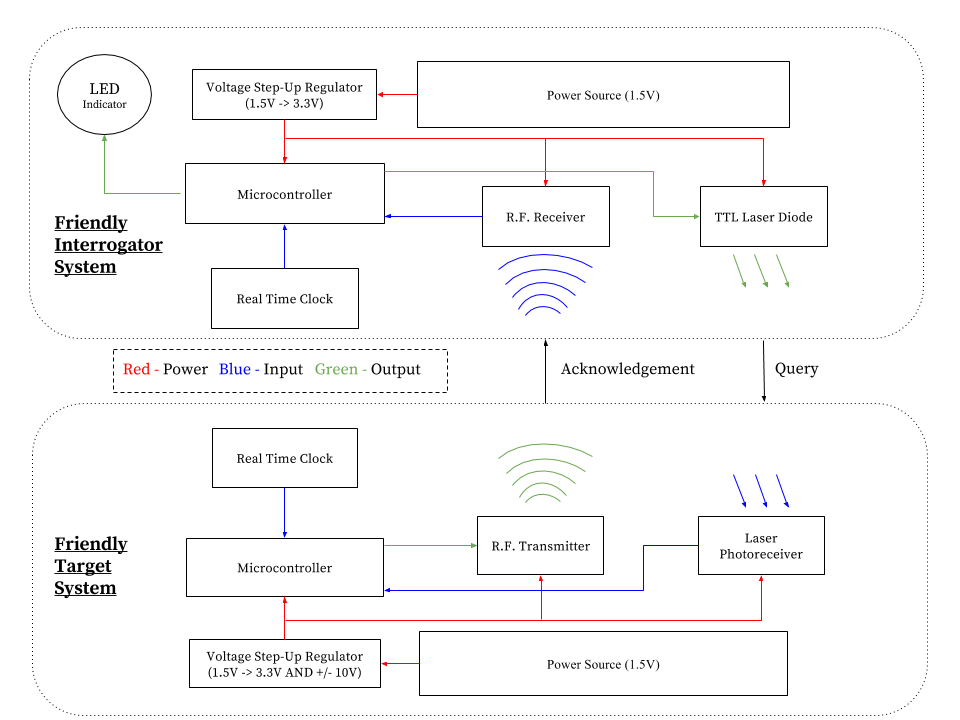
\includegraphics[scale=0.45]{System_Block_Diagram.png}
	\caption{System Block Diagram\label{fig:system-block-diagram}}
\end{figure}

The two-way communication system on both units is further divided into two one-way communication channels. The laser transmitter on board the friendly interrogator sends a signal to the photoreceivers on the friendly target. The R.F. transmitter on board the friendly target will then send acknowledgement back to the friendly interrogator. 

An important aspect of this project is encryption and ensuring an enemy cannot pose as friendly to the interrogator. This is addressed in two ways; both systems contain a locally synced clock so that a friendly target can only validate their acknowledgment within a period of time. This eliminates the possibility of an enemy intercepting and retransmitting an acknowledgment signal. Second, the acknowledgment that is sent back to the interrogator is a function of a common passphrase only know to the two systems.

%SECTION - DESIGN
\section{Design}

%DESIGN PROCEDURE
\subsection{Design Procedure} 

\subsubsection{Friendly Interrogator}
\begin{figure} [H]
	\centering
	\includegraphics[scale=0.1]{interrogator_picture.png}
	\caption{Friendly Interrogator Unit\label{fig:interrogator-picture}}
\end{figure}

\hspace{5mm}\textbf{Laser Transmitter} \label{section:laser-transmitter-design-procedure}

For safety reasons, the maximum allowable power for the laser diode is $5mW$; which registers as a Class IIIa laser. The laser diode must also fall in the visible range, so that it will trigger a person's blinking reflex before eye damage occurs. Specifically, the team used a 5 mW red 635 nm laser diode to transmit the unique I.D. (as specified by the 8-pin switch) to the friendly target. 

This laser was placed inside of a casing made out of hollow aluminum tube that was created to allow the user to adjust the spot size on the laser dot. The laser can be seen in Figure \ref{fig:interrogator-picture}. The laser diode, sourced by a transistor, allows for pulsing of a unique identification number at $5kHz$. The limiting factor for the $5kHz$ requirement was the processing speed of the MSP430 microcontroller; between every sampling of the photoreceiver, a significant amount of processing must occur. 

\hspace{5mm} \textbf{Adjustable Focus}

Adjustable focus is achieved by placing a convex lens in series after a concave lens. The convex lens is then moved to increase (or decrease) the distance between the lenses. This changes the effective focus. The effective focus of the dual-lens system can be described by Equation \ref{eq:focal-length}.

\begin{equation} \label{eq:focal-length}
	\large
	f = \frac{1}{f_1} + \frac{1}{f_2} - \frac{d}{f_1 f_2}
\end{equation}

Where $f$ is the effective focus, $f_1$ is the focal length of the concave lens (negative), $f_2$ is the focal length of the convex lens (positive) and $d$ is the distance between the lenses. 

Furthermore, the required focal length for this project is seen in Equation \ref{eq:tan}.

\begin{equation} \large \label{eq:tan}
	Tan(\theta) = \frac{r}{D}
\end{equation}

$D$ is the distance to the target, and $r$ is the radius of the beam at that distance. 

Following from these equations, Equation \ref{eq:derived-focal} can be derived.

\begin{equation} \large \label{eq:derived-focal}
	f = \frac{Dw}{r} =  \frac{1}{f_1} + \frac{1}{f_2} - \frac{d}{f_1 f_2}
\end{equation}



The adjustable focus laser has at least $\frac{1}{2}$ inches of adjustable distance. The beam width for the laser is around $2mm$. The spot radius is $20cm$. In order to test indoor in close quarters (i.e. the lab), the full distance should reach a spot radius of $20cm$ at $20 m$. At the shortest distance the spot radius should be $20cm$ at $300m$. Note that the lenses were ordered under the assumption of $50, 150, 300 m$ requirements, and so these calculations are geared towards those original requirement. This is not necessarily a bad thing, as the system is extensible to work at the original ranges which accurately reflect different combat scenarios. The requirements calculated for the adjustable focus laser are built from teh $50, 150, 350 m$ distance requirements.

This gives us a system of equations with two unknowns, shown in Equation \ref{eq:system}. 

 \begin{align} \label{eq:system} \large \begin{split}
\frac{300*.002}{0.2} =  \frac{1}{f_1} + \frac{1}{f_2} - \frac{0}{f_1 f_2}
 \\
 \frac{20*.002}{0.2} =  \frac{1}{f_1} + \frac{1}{f_2} - \frac{0.0127}{f_1 f_2}
 \end{split}
 \end{align}

Solving these equations we get the following numbers for the required focal lengths.
\begin{center}
	\large
	$f_1 \approx -53mm$ \\
	$f_2 \approx  52mm$
\end{center}

The best lenses the team could find with matching diameters were $-51mm$ and $50mm$, respectively. These calculations were originally performed under the expectation of using PVC pipes with a $\frac{1}{2}$ inch screwing distance. An updated design, explored more in depth in Section \ref{section:interrogator-adjustable-focus-laser}, allowed for several inches of adjustable distance, which more than fulfilled the requirements. 

The hardware and construction of the adjustable focus laser is discussed in greater detail in Section \ref{section-design-details}. 

\hspace{5mm}\textbf{Laser Safety}

 To achieve the laser beam diameter at $300 m$ associated in the proposal, a Class 3B laser would be required. In the State of Illinois, a Class 3B laser must be registered with the Division of Nuclear Safety in the Illinois Emergency Management Agency. The 3B laser would also present a significant viewing hazard; especially in an application where the laser is intended to be pointed at people. Since the lasers were ordered prior to the change in distance requirements, the team continued to use the $5mW$ lasers for the duration of the project. $5mW$ visible lasers have a low chance of injuring the eye, as the blinking reflex will save a victim from permanent damage; as opposed to IR lasers which can go unnoticed for several seconds. 
 
 The following is a calculation for the nominal ocular hazard distance (NOHD) of the laser, as defined by the ANSI Standard\textsuperscript{\cite{ANSI}}.
 
 The maximum permissible exposure (MPE), as defined by the ANSI Standard \textsuperscript{\cite{ANSI}} is the highest power or energy density of a light source that is considered safe, i.e. that has a negligible probability for creating damage. This MPE for a pulsing laser is calculated as the minimum of the following three rules:
 
 \begin{enumerate}
 	\item Any single pulse in the train must not exceed the MPE for the pulse exposure time.
 	\item The exposure from any group of pulses delivered in time T must not exceed the MPE for
 	time T, where T is 0.25 seconds (from the blinking reflex), for a visible laser. 
 	\item For thermal injury, the exposure for any single pulse within a group of pulses must not
 	exceed the single-pulse MPE multiplied by a multiple-pulse correction factor
 \end{enumerate}
 
 The laser will pulse at a rate of $5 kHz$. Assuming at most a 50\% duty cycle, each pulse will be of max length $1*10^{-4} s$. The divergence of the beam is smallest for the longest range; a lower divergence is more restrictive in terms of safety, so this calculation uses $300m$. Note that even though the requirements changed to $30m$, that the laser is still able to achieve the divergence necessary to reach $300m$. Thus, since the device can have a minimum divergence to reach $300m$, the safety limitations are calculated at this divergence. 
 
 At $5mW$ with a pulse width of $1*10^{-4}$, the power of the laser is $5*10^{-7} J$. 
 
 ANSI defines several constants for use in the calculation of laser safety. The relevant constant for these calculations is the constant $C_6$. This is defined as Equation \ref{eq:c6-equation}.
 
 \begin{align} \label{eq:c6-equation} \large \begin{split}
 C_6 =\frac{\theta}{1.5} \hspace{5mm} for \hspace{2.5mm}(1.5 \leq \theta \leq 100)
 \\
 C_6 = 1 \hspace{5mm} for \hspace{2.5mm} ( \theta < 1.5, \theta > 100)
 \end{split}
 \end{align}
 
 Using trigonometry, the divergence angle, $\theta$, for the laser is shown in Equation \ref{eq:div-angle}.
 
 \begin{equation}\label{eq:div-angle} \large
 \theta = Tan^{-1}(\frac{r}{300})* 1000 [mrad]
 \end{equation}
 
 Following the ANSI standard, the Rule 1 calculation is shown in Equation \ref{eq:r1}.
 \begin{equation}\label{eq:r1}
 \large
 R_1 = 5*10^{-3} * C_6
 \end{equation}
 
 The Rule 2 calculation is Equation \ref{eq:r2}.
 \begin{equation}\label{eq:r2}
 \large
 R_2 = 18 (T)^{0.75}
 \end{equation}
 
 The Rule 3 calculation is Equation \ref{eq:r3}.
 \begin{equation} \label{eq:r3}
 \large
 R_3 = R1(T*f)^{0.25}
 \end{equation}
 
 The most restrictive rule defines the MPE as Equation \ref{eq:mpe}.
 \begin{equation}  \label{eq:mpe}
 \large
 MPE = min(R_1, R_2, R_3)
 \end{equation}
 
 The MPE, then, is the following.\\
 {\large $min($}
 \begin{center}
 	\large
 	$5*10^{-3} * Tan^{-1}(\frac{.5}{300})* 1000$,\\
 	$18 (.25)^{0.75}$,\\
 	$0.00833333 (0.25*5000)^{0.25}$
 \end{center}
 {\large $)$}
 
 This gives the following.
 \begin{center}
 	\large
 	$MPE = min(0.00833333, 6.36396, 0.0833333) = 0.00833333 [\frac{J}{m^2}]$
 \end{center}
 
 The NOHD is defined as Equation \ref{eq:mpe-2} (with $\theta$ in terms of $rad$, not $mrad$).
 \begin{equation} \large \label{eq:mpe-2}
 \frac{\sqrt{\frac{4 * P}{\pi * MPE}} - 2w}{\theta}
 \end{equation}
 
 Where P is the power of the beam ($5*10^{-7} J$) and $w$ is the waist of the beam, $0.5mm$. This gives an NOHD of 
 \begin{center}
 	\large
 	$ \frac{\sqrt{\frac{4 * 5*10^{-7} }{\pi * 0.00833333}} - 2*0.0005}{Tan^{-1}(\frac{.5}{300})} = 4.64m$
 \end{center}
 
 The team took precautions to avoid eye contact with the laser within $5 m$ of the source, and kept a wide divergence angle when possible. If it was absolutely necessary to work with the laser powered on at full divergence, and a person within $5m$ of the laser, the person wore protective eye wear. 
 
 The risk of eye damage was mitigated by the fact that the laser is both visible, not always powered on, and adjustable to have a very wide divergence. 

\subsubsection{Friendly Target}


\begin{figure} [H]
	\centering
	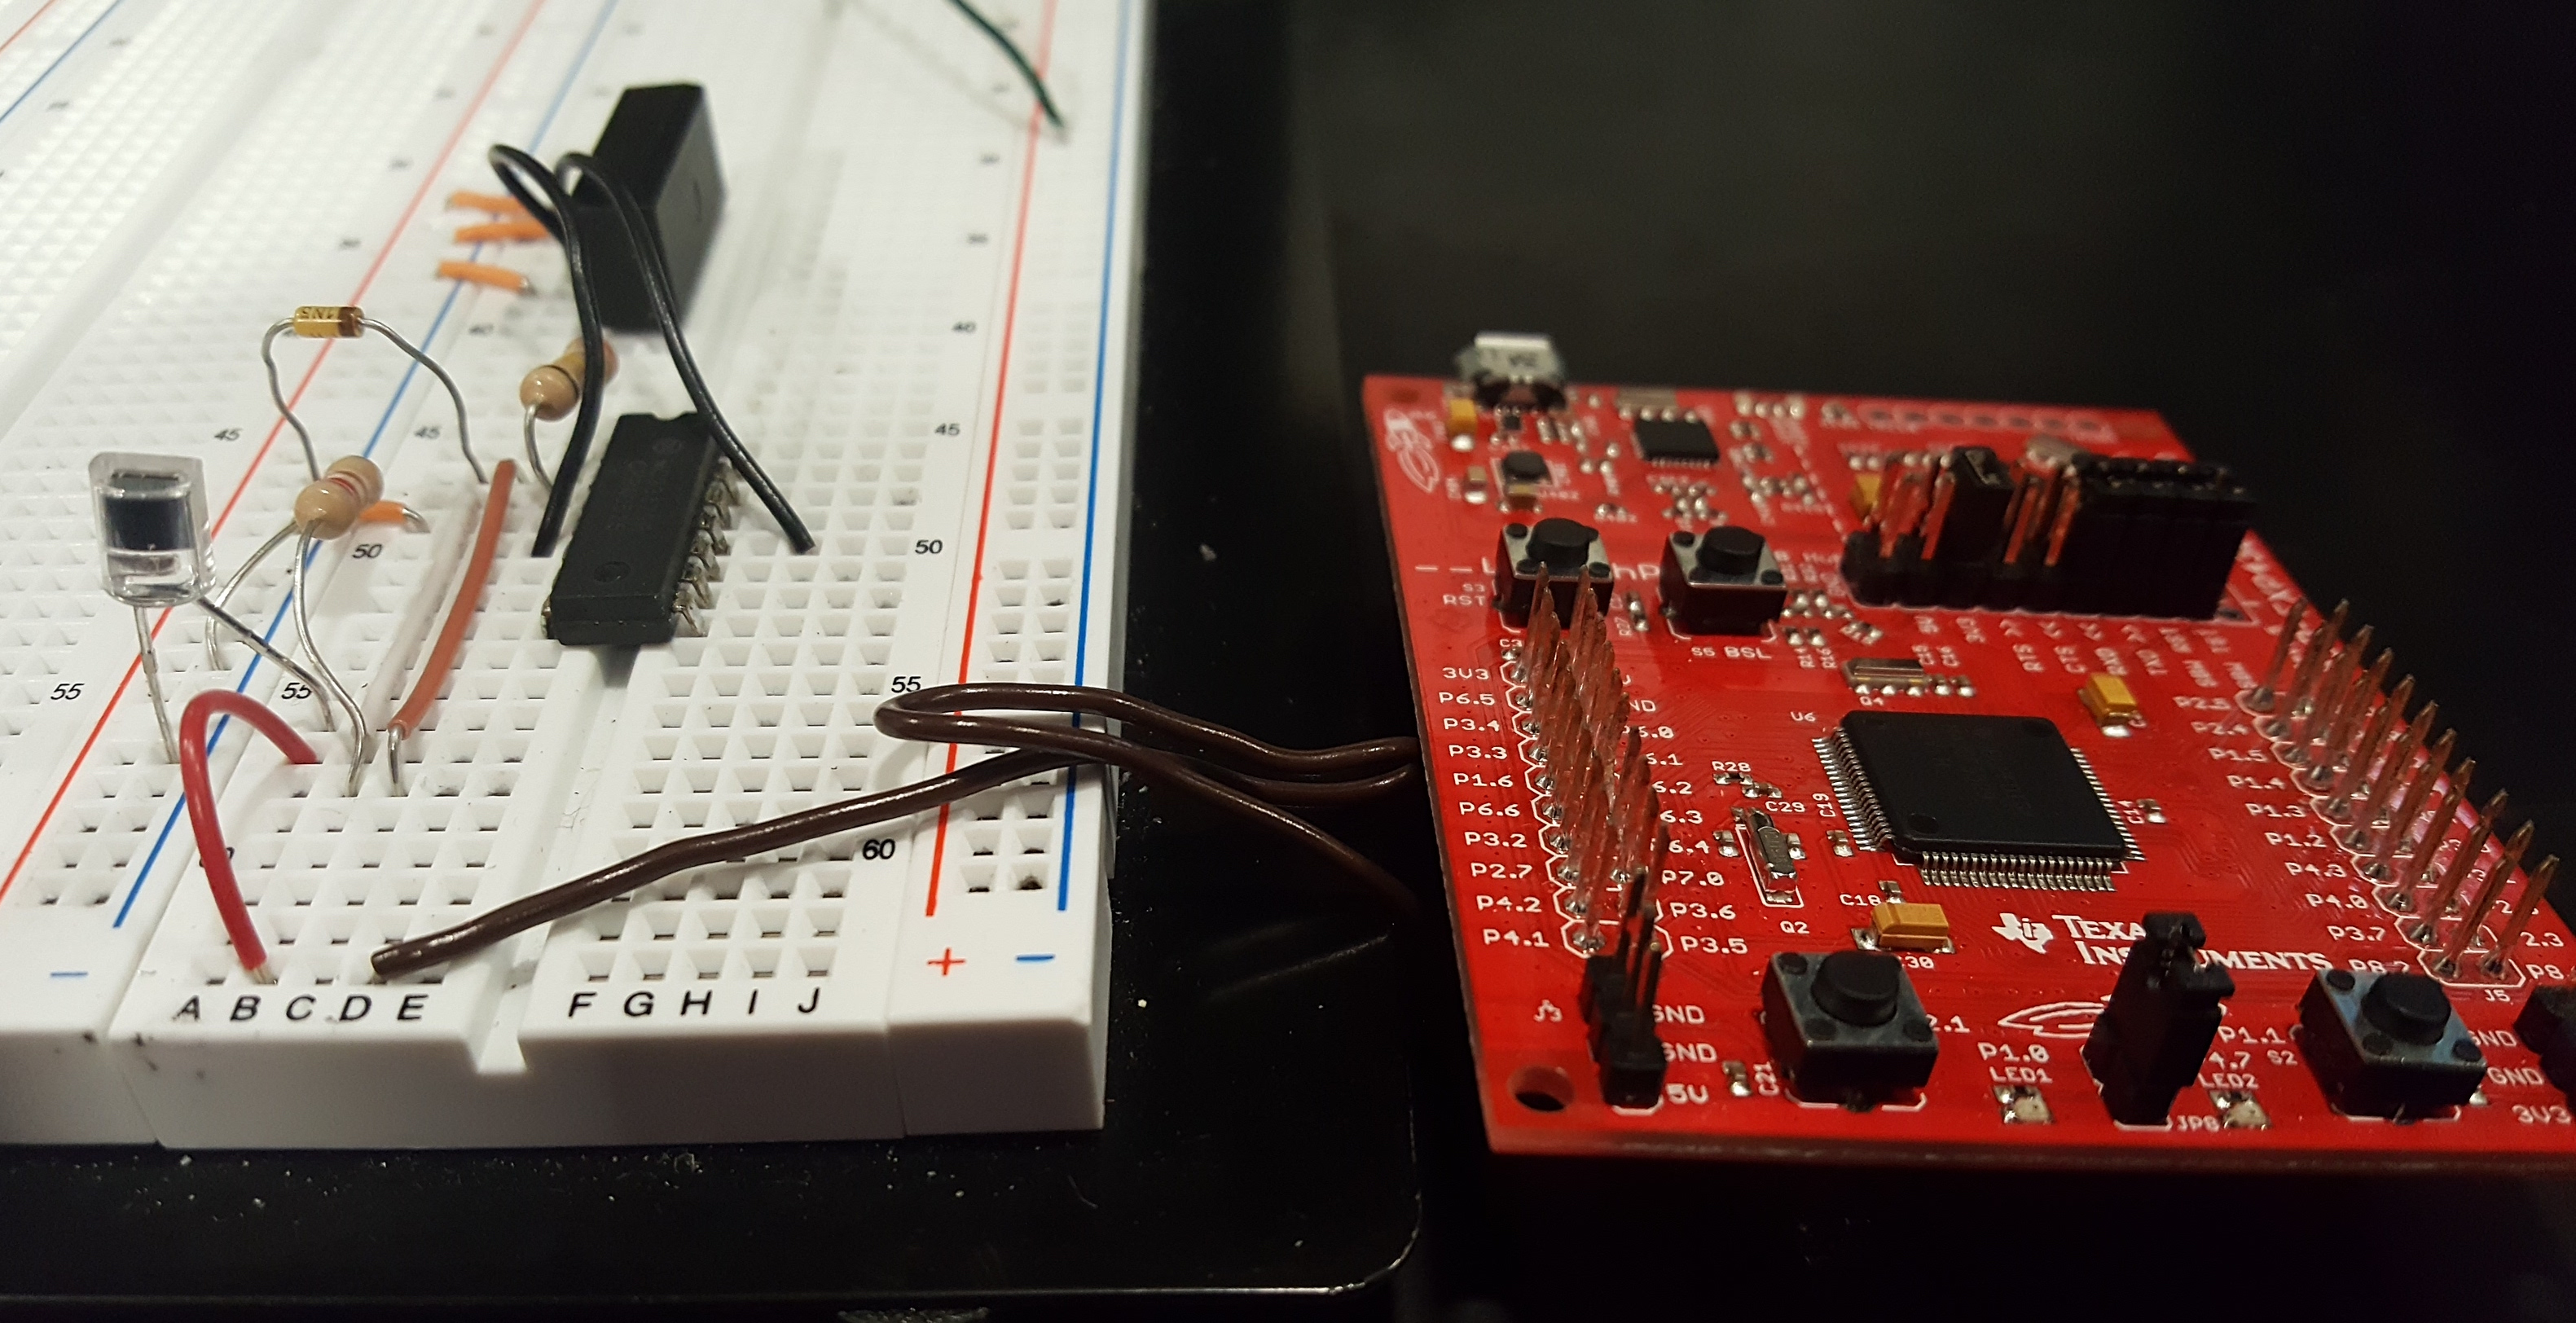
\includegraphics[scale=0.08]{target_picture.png}
	\caption{Friendly Target Unit\label{fig:target-unit}}
\end{figure}


\hspace{5mm}\textbf{Laser Photoreceiver} \label{section:laser-photoreceiver-design-procedure}\\
A photodiode was chosen such that a 5kHz signal could be processed and boosted to register a value between 0 and 3.3V at a maximum distance of $30m$ from the laser source. This couples the photoreceiver requirement with the intensity of the laser diode, which is capped at $5 mW$. 

The inherent limitations of laser power for safety means that the performance is in the hands of the photodiode. The team did not change their design review choice and selected PIN photodiodes as they have a high sensitivity and speed.

One of the selection criteria for the photodiodes was the material with which the photodiode is made. This includes materials such as Si, InGaAs, and InA. The optimum wavelength is dependent on the material selection.

With photodiodes, noise-equivalent power (NEP) is a measure of the incident power required to generate a response signal equal to the noise level of a detector system. Detectivity is the reciprocal of the NEP normalized for the active area of the photodiode.\textsuperscript{\cite{Microphotonics}}. The best photodiode, then, had the highest detectivity for the visible wavelength.  

\begin{figure} [H]
	\centering
	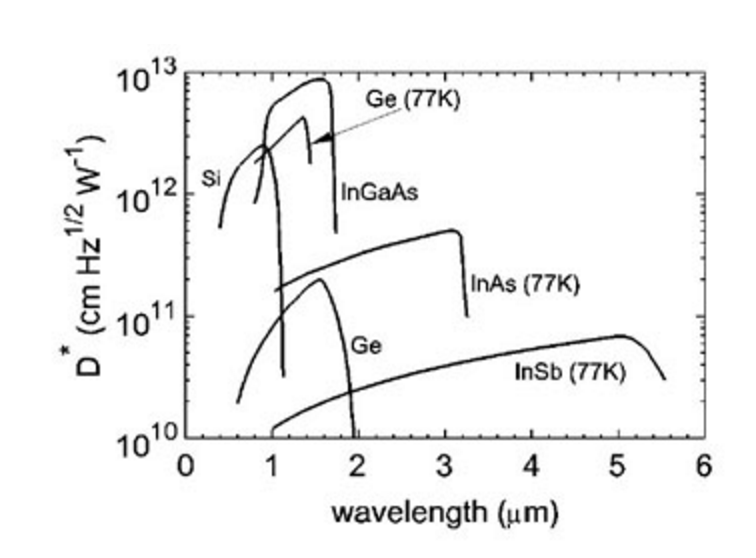
\includegraphics[scale=0.4]{detectivity-table.png}
	\label{fig:detectivity-table}
	\caption{Specific Detectivity for Photodetector Materials \textsuperscript{\cite{Optical}} \label{fig:detectivity-table}}
\end{figure}

Figure \ref{fig:detectivity-table} illustrates the specific detectivity ranges of photodiodes. The interrogation laser is in the visible range; therefore, the matching photodiode was of type Si. Using this type of photodiode, the detectivity is between $10^{10}$ and $10^{13}$ $\frac{Hz^{\frac{1}{2}}}{W}$. The following calculations use a conservative value, $10^{12} \frac{Hz^{\frac{1}{2}}}{W}$, as the detectivity. In realty, because the wavelength is less than \SI{1}{\micro\meter}, the detectivity is somewhere between $10^{12}$ and $10^{13}$ $\frac{Hz^{\frac{1}{2}}}{W}$

The equation for NEP from detectivity, $D^*$, and photodiode active area, $A$,  is Equation \ref{eq:nep}.
\begin{equation} \large  \label{eq:nep}
	NEP = \frac{\sqrt{A}}{D^*}  [\frac{W}{Hz^{1/2}}]
\end{equation}

The incident irradiance, $E_i$, to cancel noise is Equation \ref{eq:ei}.
\begin{equation} \large  \label{eq:ei}
	E_i = \frac{NEP * \sqrt{f}}{A} = \frac{\sqrt{Af}}{AD^*} = \frac{f}{D^*\sqrt{A}} [\frac{W}{m^{2}}]
\end{equation}

The NEP measures the incident irradiance to cancel the noise on the photodiode. To register a signal on the MCU, the incident irradiance must be higher than the noise. To be conservative, define the required incident irradiance as Equation \ref{eq:ereq}.
\begin{equation} \large \label{eq:ereq}
	E_{req} = 2E_i [\frac{W}{m^{2}}]
\end{equation}

Multiplying the area of the laser's spot by the required incident irradiance at the photodiode gives the necessary power. Thus, the radius of the spot in terms of the power of the laser and required incident irradiance at the photodiode is shown in Equation \ref{eq:r}.
\begin{equation} \large \label{eq:r}
	r = \sqrt{\frac{P}{\pi E_{req}}} [m]
\end{equation}

Note that the power contained in the laser's spot does not depend on distance from the source, as atmospheric reflection is negligible at $30 m$.

The radius, in terms of the detectivity, frequency, and sensor active area is in Equation \ref{eq:r-2}.
\begin{equation}\large \label{eq:r-2}
	r = \sqrt{\frac{PD^*\sqrt{A}}{2 \pi f}} [m]
\end{equation}

The design review/proposal listed $0.8382 m$ as the ideal radius of the laser's spot. Unfortunately, with the $5mW$ red laser, this would require a sensor with a massive active area. The largest sensor the team could find, at a reasonable price, has a $8.53 mm^2$ active area. 

For the $8.53 mm^2$ active area photodiode operating at $635 nm = 4.72441 × 10^{14} Hz$, the radius should be the following.
\begin{center}
	$r = 0.326998 m \approx 33 cm$
\end{center}

This theoretical working spot radius for receiving a signal is large enough for such a system to be plausible; thus, the chosen photodiode was more than sufficient. 

\subsubsection{System}

\hspace{5mm}\textbf{R.F. Transmitter/Receiver} \label{section:rf-transmitter-design-procedure} \\
The team purchased the Linx KH3 R.F. transmitter/encoder and receiver/decoder with the intentions of it being relatively easy to use out of the box and easily programmable with any MCU. However, in reality, the receiver proved to be much more difficult than the team imagined. 

Surface mount device (SMD) adapters were used to plug the R.F. receiver into a breadboard and soon thereafter, the team learned that breadboards act as a large capacitor and filter out lower frequencies, which made the team question the reliability of testing with 315MHz. For this reason, the team switched to using perf boards and soldering female connections to connect to the SMD adapter. 

This caused many problems with establishing a reliable connection and soldering this equipment to a board for the first time was especially difficult. As explained in Section \ref{section-design-details}, the R.F. transmitter/receiver did not work in the end of the project due to equipment defectiveness.

The requirement driving both the R.F. transmitter and receiver was the ability to broadcast and receive packets (as a pair) at the maximum distance of the project ($30m$). The theoretical maximum distance was explored in the design review and thus are not be discussed here. On both the friendly interrogator printed circuit board (PCB) and the target PCB, the 3.23mm (50 $\Omega$) microstrip line was fabricated (using the same equations as the design review \textsuperscript{\cite{Microstrip}}), but not used in the final implementation.


\hspace{5mm}\textbf{Voltage/Power Regulation} \label{section:interrogator-voltage-regulation-design-procedure}

It is required that the power stay above 3.3V for a period of 8 hours. Originally, in the design review, a 3.3V boost-converter was going to be utilized along with a single AA battery (1.5V) to supply the entire interrogator unit. This proved to be a difficult implementation to use due to the MSP drawing more power than the team expected at the time of the design review. Also, the PCB mounting of this equipment proved to be difficult for unexperienced solderers. 

For this reason, the team opted to use four AA standard alkaline batteries put through a regulator to drop the voltage supplied to the PCB down to 3.3V. 

In the friendly interrogator, this 3.3V output is fed directly into the MSP and R.F. modules for power.

In the friendly target, this 3.3V output is fed to the MSP and R.F. modules, and is also routed through a boost converter to $\pm 12V$, which in turn powers the photoreceiver op-amp. The photoreceiver draws significantly more power under heavy light from the laser because of it's clipper circuit; in actual use, this concentration of light rarely happens. 

 
\hspace{5mm}\textbf{Microcontroller} \label{section:system-design-procedure}

The microcontroller needed to have enough ports to service both the R.F. boards and laser/photoreceiver inputs, have enough speed to sample and decide on a packet value received at $5kHz$, and have the ability to count seconds. A vast majority of microcontrollers fit the requirements for this, as most come with several ports, fast processors, and a built in timer.

In the design review, the team was using a MSP430F2274IDA, which proved to be very difficult to program using the lab-supplied FET programmer. For this reason the team decided to switch to the MSP432P401R(Launchpad model MSPEXP432P401) which contained an onboard debugger. These were much easier to use due to the USB-to-microUSB debugger. The team used these microcontrollers for approximately two weeks until both boards were determined to be defective due to internal shorts (drawing approximately 0.5A standby -  should be drawing ~4mA \textsuperscript{\cite{MSPEXP432P401R}}).

The team then decided to switch back to the MSP430 line but instead decided to use the Launchpad series similar to the MSP432. The MSP430G2553 (Launchpad model MSP-EXP430G2) was ultimately the model the team used during final demonstration. These worked excellent and did not cause any problems during demo. 

Other microcontroller options, including PIC and arduino were considered. Arduino was considered overkill and low difficulty for the project, PIC more difficult to work with due to less documented proprietary systems. If pursuing this project further, the team would have still chosen the MSP430 Launchpad series due to the familiarity of using them for the 8 weeks during this project.


%DESIGN DETAILS
\subsection{Design Details} \label{section-design-details}


\subsubsection{Friendly Interrogator}

\hspace{5mm}\textbf{Adjustable Focus Laser}
\label{section:interrogator-adjustable-focus-laser}

The adjustable focus laser was built using two lenses, one convex and one concave. The laser can be seen in Figure \ref{fig:laser-transmitter}.

\begin{figure} [H]
	\centering
	\includegraphics[scale=0.05]{laser-transmitter.png}
	\caption{Laser Transmitter \label{fig:laser-transmitter}} 
\end{figure}

The concave lens is mounted in a 1/2 inch PVC nipple with hot glue. Behind the lens, a cut acrylic cicle with a hole in the center holds the laser in place. This acrylic cutout is also hot glued in place.

The acrylic cutout holding the laser in the PVC nipple can be seen in Figure \ref{fig:acrylic}.

	\begin{figure}%
		\centering
		\subfloat{{\includegraphics[width=5cm]{acrylic.png} }}%
		\qquad
		\subfloat{{\includegraphics[width=5cm]{nipple.png} }}%
		\caption{Acrylic Laser Holder in PVC Nipple}%
		\label{fig:acrylic}%
	\end{figure}
	
Using electrical tape to create a tight fit, the PVC nipple rests inside a sawed-off shower curtain rod. At the very end of the rod, the concave lens is secured in place using hot glue and a PVC connector. This can be seen in Figure 7.

\begin{figure} [H]
	\centering
	\includegraphics[scale=0.05]{end.png}
	\caption{Concave Lens Secured by PVC Connector	\label{fig:end}}
\end{figure}

The shower curtain rod allows a user to twist counter-clockwise to free lateral motion, and then twist clockwise to secure the rod in place. This was ideal for the purpose of the interrogator's adjustable focus laser, as a user can adjust the focus and secure the rod in place. Figure 8 shows a picture with the rod fully extended, which shows a much larger length than the picture in Figure 5.

\begin{figure} [H]
	\centering
	\includegraphics[scale=0.05]{extended-rod.png}
	\label{fig:extended}
	\caption{Extended Adjustable Focus Laser}
\end{figure}

\hspace{5mm}\textbf{Circuit Schematics \& PCB} \label{section:interrogator-circuit-schematics-design-details}
The circuit and PCB evolved a great deal from the design review to simplify the system. First, the MSP microcontroller was changed from a surface mount device to a breakout using pinheaders on the PCB. The crystal oscillator circuit was removed and some switches were removed due to their complexity.

The PCB adhered to the guidelines set out by the ECE Service Shop \textsuperscript{\cite{ECE-Electronics-Shop}}.
Please refer to Figure \autoref{fig:interrogator-schematic} for the circuit schematic of the friendly interrogator unit and Figure \autoref{fig:interrogator-pcb} for the PCB layout of the friendly interrogator unit. 



\subsubsection{Friendly Target}
\hspace{5mm}\textbf{Circuit Schematics \& PCB} \label{section:target-circuit-schematics-design-details}

Please refer to Figure \ref{fig:target-schematic} for the circuit schematic of the friendly target unit.  Please refer to Figure \ref{fig:target-pcb} for the pcb layout of the friendly target unit. 

\hspace{5mm} \textbf{Software} \label{section:target-software-design-details}\\
Incoming transmissions are broken into two parts, where a $1$ corresponds to a high at the transmission source, and a $0$ a low. These two parts are shown below:
\begin{enumerate}
	\small
	\item \textbf{Preamble} - $10101010$ 
	\item \textbf{Packet} - An 8 digit long value representing a numerical id
\end{enumerate}

Values from the photoreceiver are analog values ranging from $0-3.3V$. Because the ambient light in the room, the photoreceiver can report $0-2V$ when receiving no light from the transmitter. For this reason, an algorithm was created to decide binary values of a transmission based only on the \textit{difference} between the current analog value and the analog value $200 \mu s$ before. This is similar to Non-Return to Zero Inverted (NRZI) encoding scheme widely used in many applications. This is Algorithm \ref{algo-1} shown in the appendix.  Figure \ref{fig:threshold} elaborates on the threshold noise difference. The top two dotted lines represents the variations in the "high" signal, and the bottom two dotted lines represent the variations in a "low" signal. These must be accounted for in the software.

\begin{figure} [H]
	\centering
	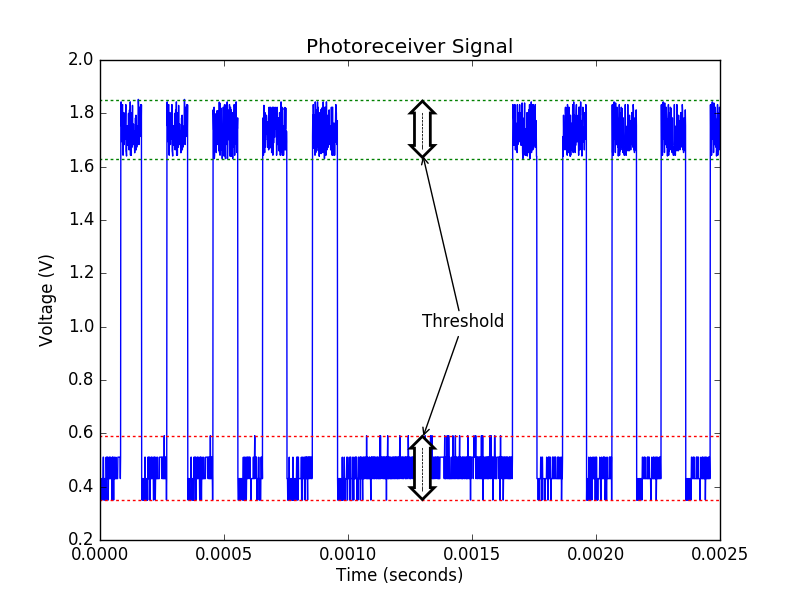
\includegraphics[scale=0.45]{threshold.png}
	\caption{Threshold Noise Difference\label{fig:threshold}}
\end{figure}


Binary values are stored in an array of length 8, since both packets and preambles are 8 bits. Because a preamble can come at any moment, an algorithm was designed both to store binary values in the array, and to always check for a preamble packet. This is Algorithm \ref{algo-2} in the appendix.

Once a preamble has been received, a simple algorithm is used to capture a packet. This is Algorithm \ref{algo-3} in the appendix. After 100 queries of a packet has received 85\% success, an acknowledgment will be sent over R.F.

\subsubsection{R.F. Receiver/Transmitter}
As stated previously, the R.F. equipment was determined to be defective after establishing the standby current was 15 times the value provided by the datasheet (standby was supposed to be 10 mA, received 150mA\textsuperscript{\cite{Linx-Transmitter}\cite{Linx-Receiver}}). This could have been the result of neglect by the team or improper soldering (i.e. soldering/desoldering multiple times). Either way, unfortunately the team was unable to carry forth with the design implementation of the R.F. receiver/transmitter and therefore did not perform verification.

%SECTION - VERIFICATION
\section{Verification}

The Requirements and Verification Table is shown in the back of the appendix.


\subsection{Laser Transmitter \& Photoreceiver}
\subsubsection{Distance Requirement}
Table \ref{tab:distance-requirement} displays the values received on a digital multimeter when performing the verification for the distance requirement. 
\begin{table}[htbp]
	\centering
	\begin{tabular}{c|c|c}	% ccccccc indicates 7 center aligned columns
		\toprule	% top separator
		Distance & Ambient & Transmitter On \\
		\midrule
		2 m  & 0.556 V & 1.75 V\\
		5 m & 0.526 V & 1.59 V\\
		15 m & 0.636 V & 1.12 V\\ 
		30 m & 0.562 V & 0.87 V\\
		
		\bottomrule	% bottom separator
	\end{tabular}%
	\caption{Laser Transmitter Distance Test}
	\label{tab:distance-requirement}	% this is the label given to the table that can be referenced using \ref{tab:Exp1Part1_7}
\end{table}%

\subsubsection{Spot Size Requirement}
Table \ref{tab:spot-size} displays the values received when measuring the spot size of the laser transmitter during the verification of the spot size requirement. 
\begin{table}[htbp]
	\centering
	\begin{tabular}{c|c|c}	% ccccccc indicates 7 center aligned columns
		\toprule	% top separator
		Distance & Smallest Spot Size Radius & Largest Spot Size Radius \\
		\midrule
		2 m  & 1.5mm & 16.2mm\\
		5 m & 3.75mm & 36.5mm\\
		\bottomrule	% bottom separator
	\end{tabular}%
	\caption{Laser Transmitter Spot Size Test}
	\label{tab:spot-size}
\end{table}%

\subsubsection{Packet Reception}
The top half of Figure \ref{fig:packet-verification} shows the signal that was sent through the MCU to the laser, and the bottom half of the same figure shows the received signal by the photoreceiver after amplification. Both signals are sent and received at a 5kHz rate and the voltage is sufficient enough to be detected by an ADC on board the MCU. 
\begin{figure} [H]
	\centering
	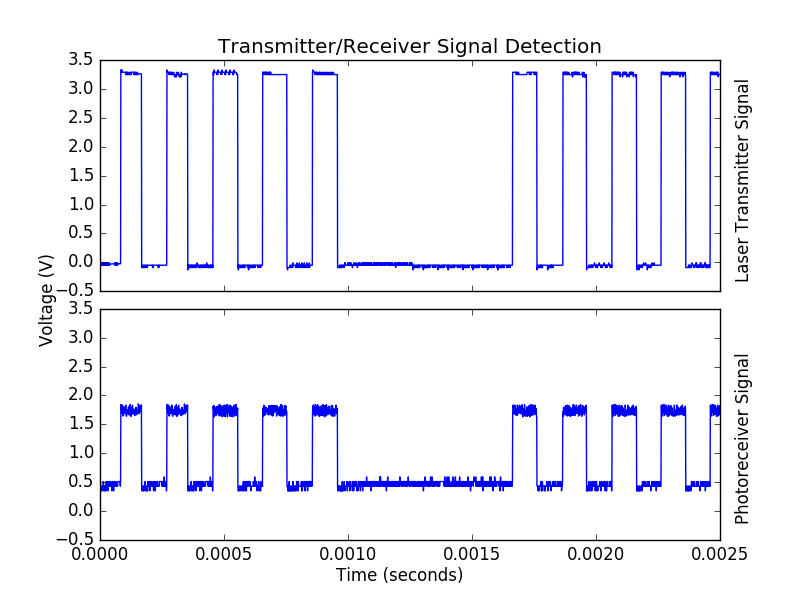
\includegraphics[scale=0.45]{packet_verification.png}
	\caption{Packet Sent/Received Signal\label{fig:packet-verification}}
\end{figure}

\subsubsection {Counting Packets}
Algorithm \ref{algo-4} was used to count the number of missed packets from the photoreceiver.
The results are shown in Figure \ref{fig:transmitted-received}. The algorithm verified at 5 meters, over 85\% packet reception. The requirement is the blue dotted line, and the last bar is the average of all 10 trials (which turned out to be 86\%).

\begin{figure} [H]
	\centering
	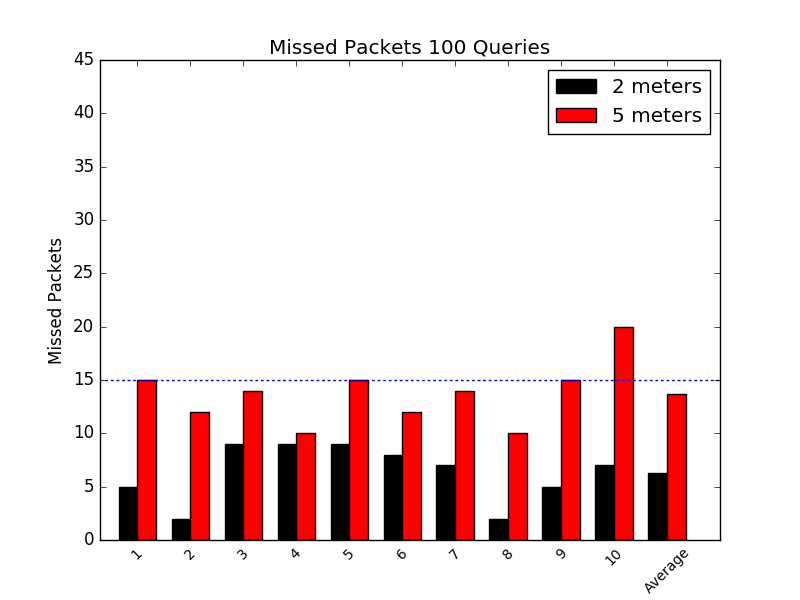
\includegraphics[scale=0.45]{transmitted_received.png}
	\caption{Missed Packets Verification\label{fig:transmitted-received}}
\end{figure}

\subsection{R.F. Transmitter \& Receiver}
As stated previously, the R.F. modules were determined to be defective before any verification could be performed. For this reason, this section will be omitted. 

\subsection{Power Module}
The requirements stated the power module needed to output a steady 3.3V for a period of 8 hours $\pm$ 5\%.

\hspace{5mm}\textbf{Friendly Interrogator Consumption} \label{section:interrogator-consumption}
\begin{table}[H]
	\centering
	\begin{tabular}{c|c}	% ccccccc indicates 7 center aligned columns
		\toprule	% top separator
		Module & Active Current Consumption \\
		\midrule
		MSP430 & 1.521 mA \\ 
		Linx KH3 R.F. Receiver & 10.1 mA \\
		5 mW Laser & 24.7 mA (max) \\
		PCB  & 30.1 mA \\
		\bottomrule	% bottom separator
		\textbf{Total} & 65.62 mA \\
	\end{tabular}%
	\caption{Current Consumption Values for Interrogator Unit}
	\label{tab:table2}	% this is the label given to the table that can be referenced using \ref{tab:Exp1Part1_7}
\end{table}%

Assuming a standard alkaline battery has 1500mAh on a full charge \textsuperscript{\cite{Battery}}, the total active time can be calculated as shown in Equation \ref{eq:active-time}.

\begin{equation}  \large \label{eq:active-time}
	\textrm{Total Active Time} = \frac{Total Charge On Battery}{Total Current Consumption} = \frac{1500mAh}{65.62mA} = 30.12 hours 
\end{equation}

\hspace{5mm}\textbf{Friendly Target Consumption} \label{section:ttarget-consumption}
\begin{table}[H]
	\centering
	\begin{tabular}{c|c}	% ccccccc indicates 7 center aligned columns
		\toprule	% top separator
		Module & Active Current Consumption \\
		\midrule
		MSP430 & 1.521 mA \\ 
		Linx KH3 R.F. Transmitter & 7.81 mA\\
		Photoreceiver (including voltage booster) & 52.55(min), 328.55 mA (max)\\
		\bottomrule	% bottom separator
		\textbf{Total} & 74 mA (standby), 350 mA (max) \\
	\end{tabular}%
	\caption{Current Consumption of Target Unit}
	\label{tab:table2}	% this is the label given to the table that can be referenced using \ref{tab:Exp1Part1_7}
\end{table}%

Note that the high max current consumption of the photoreceiver was acquired with the 5mW laser, fully focused 2 cm away from the photodiode. This causes a large voltage from the photoreceiver op amp, which is then clipped by a 3.3V diode. The current flow through the diode is what causes this high max. While this heavy flow is not ideal, in normal operating conditions this much light would never be present on the photoreceiver; it would take a flash bang or equipment misuse to yield this high an output. 

This yields a battery life between 5.7 and 27 hours, most likely 20+ hours, barring misuse. 

\subsection{System Speed}

This verification was unable to be performed because the system was not functioning as a whole at the time of demo. Theoretically, however, the system exceeds this requirement. 

%COSTS
\section{Costs}

The labor cost was calculated as follows:

\begin{center}
	Total Cost = Parts + Worker Salary (\$/hour) x 2.5 x Time (Hours) Invested In Project
\end{center}

\begin{figure} [H]
	\centering
	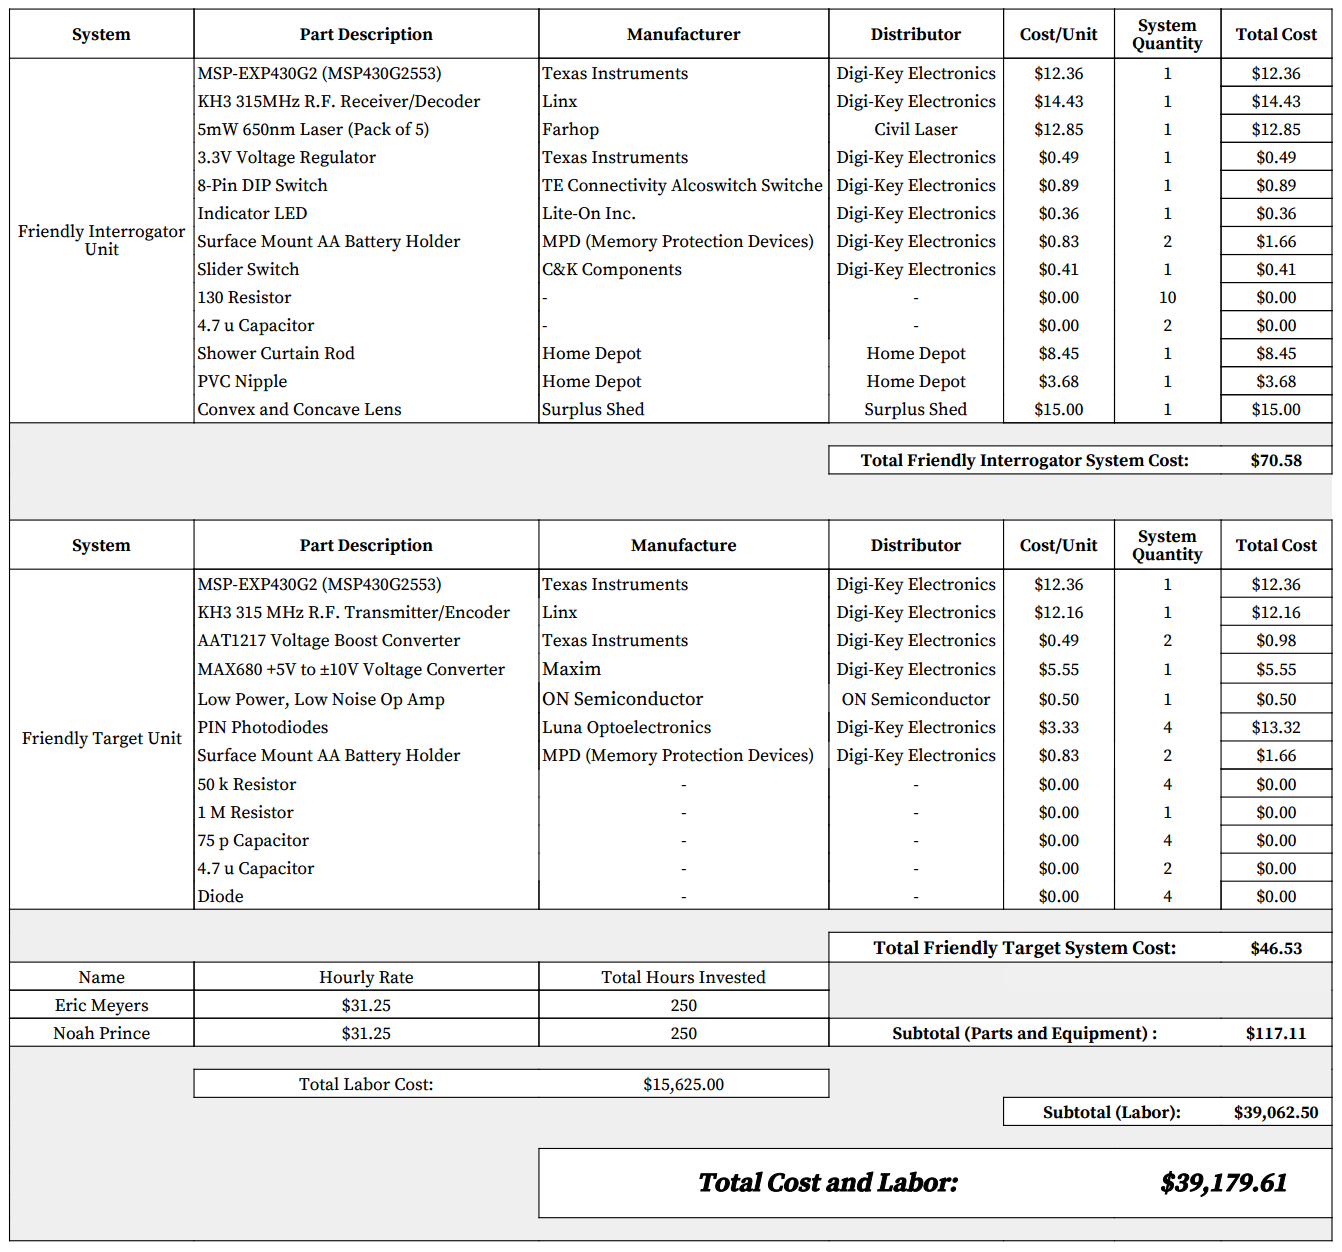
\includegraphics[scale=0.60]{parts-labor-cost.png}
	\caption{Parts and Labor Cost\label{fig:parts-labor-cost}}
\end{figure}



%CONCLUSION
\section{Conclusion}
The team learned a considerable amount over the course of this project. In addition to designing, building, and testing PCBs using EAGLE, the team also learned how to bring a project from an idea to a concrete implementation. Throughout the semester, the team bettered their abilities in key ECE skills like soldering and circuit debugging. The team learned that even when you want things to work, things never work out as planned. 

After the design review and during fabrication, the team realized that the project as a whole was a bit too complex for novice PCB designers and builders. In retrospect, the system would have been immensely simplified from the beginning. It is much easier to start from something small and build complexity a step at a time. 

The R.F. proved to be the most difficult part of this project. During design review, the team did not allocate enough time in the schedule compared to how long it would have took. The planning could have been better, and if pursuing the project further, this, hopefully would have been avoided.

The team overall did not harm anyone during this project, nor did not use any weapons, rather were simply demonstrating the effectiveness of a piece of identification equipment. An ethics section is included below to review relevant topics.

\subsection{Ethics}
The following ethical considerations refer to the IEEE Code of Ethics\cite{IEEE}.

\textit{"1. To accept responsibility in making decisions consistent with the safety, health, and welfare of the public, and to disclose promptly factors that might endanger the public or the environment"} \\
\textit{"9. To avoid injuring others, their property, reputation, or employment by false or malicious action"}

This project fully acknowledged the danger of lasers, and in the design review calculated an NOHD of $1.25m$. Another aspect of the project that could have endangered the public is the misuse of an IFF system. We want to be clear that just because a target doesn't acknowledge as "friendly" does NOT mean that the target is dangerous. As always, anyone wielding a firearm should consider both the target and the area behind the target before firing. This system is meant to supplement, not replace, good judgment.  

\textit{"2. To avoid real or perceived conflicts of interest whenever possible, and to disclose them to affected parties when they do exist"}

Our project may contain conflicts of interest in that two opposite sides of a combat scenario could use this technology. We would disclose this information to both sides. It is our hope that this technology will reduce the amount of friendly fire casualties, regardless of allegiance. 

\textit{"3. To be honest and realistic in stating claims or estimates based on available data"}

We will always be honest with the capabilities of this system. To skew the capabilities could put infantry and non-combatants in danger. 

\textit{"5. To improve the understanding of technology; its appropriate application, and potential consequences"}\\
\textit{"6. To maintain and improve our technical competence and to undertake technological tasks for others only if qualified by training or experience, or after full disclosure of pertinent limitations"}

The entire purpose of senior design is to meet these requirements. As college students, we aspire to improve ours, and other's, understanding of technology. We also fully acknowledge limitations of our abilities and will supplement with help from the course staff. 

\textit{"7. To seek, accept, and offer honest criticism of technical work, to acknowledge and correct errors, and to credit properly the contributions of others"}

We are always willing to have a dialog with those interested in are work. We also seek to correct any errors so that the project meets all requirements. In building any project, one relies heavily on work already done by others; it is important to give credit where it is due. 


\subsection{Future Work}

The system as a whole is currently not functioning due to the R.F. equipment breaking down. The team is confident that, given a proper R.F. setup, the system would function as intended. 

Future work also includes building more condensed, specialized PCBs to hold the two main modules. 

Further down the development line, mounting for both the target and interrogator unit would need to be built. On the target unit, this would mean wiring multiple photodiodes to a soldier's equipment and creating a waterproof storage pack on the soldier's person. For the interrogator unit, this would mean a weaver rail mount for the laser, and a waterproof storage pack for the circuitry (if it is not attached to the laser). Additionally, the adjustable focus laser would need to be more precise; that is, a 3D printed casing could be created to hold the laser and lenses. This casing could include screws, similar to those on a rifle scope, to fine tune the accuracy of the laser. 

\clearpage
%REFERENCES
\bibliographystyle{IEEE_ECE}
% include the BibTex file here to build reference
\bibliography{Citations}\addcontentsline{toc}{section}{Reference}
\clearpage
\section*{Appendix}
\pagenumbering{gobble}

\begin{figure} [H]
	\centering
	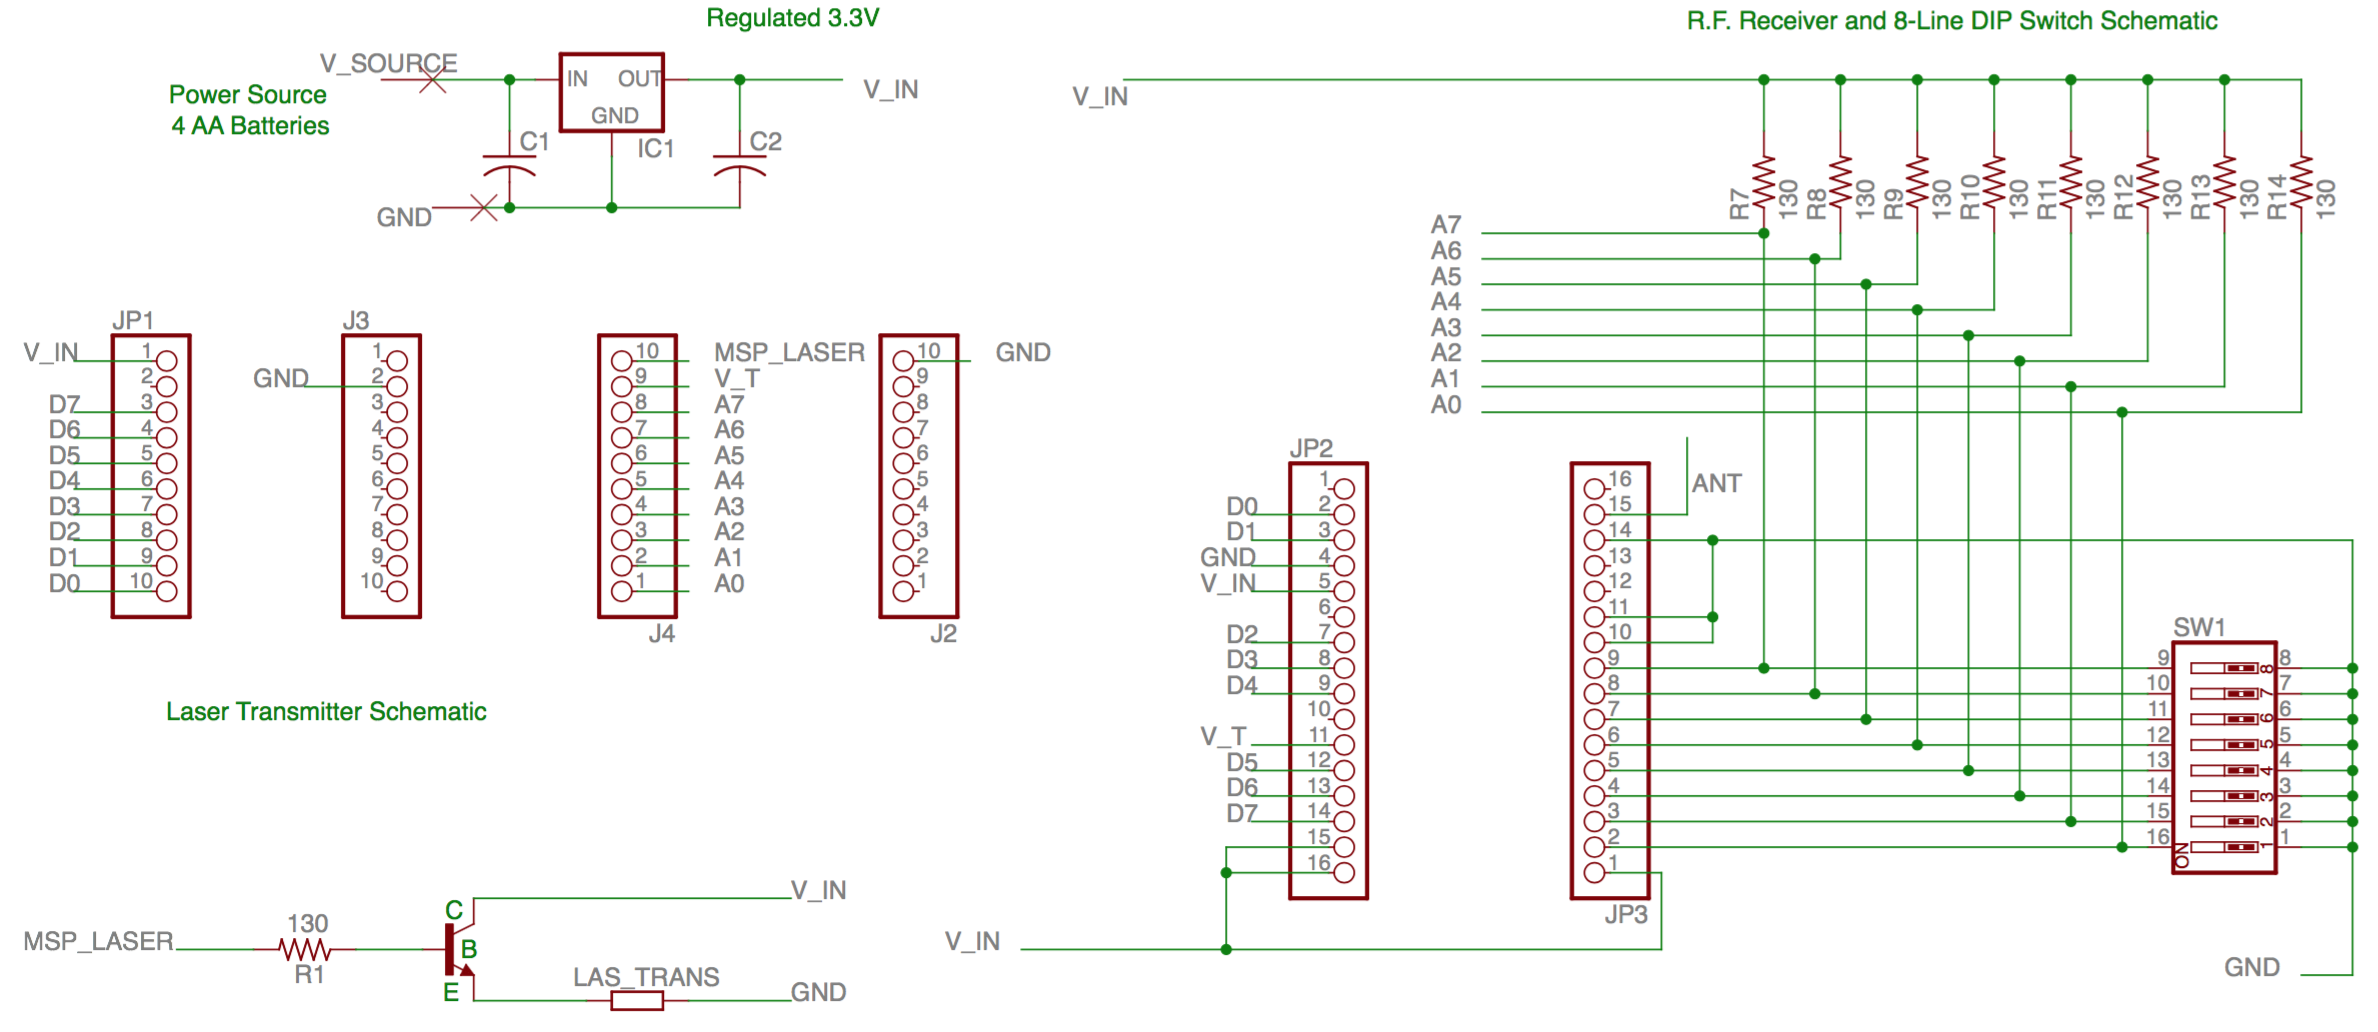
\includegraphics[scale=0.37]{friendly_interrogator_circuit.png}
	\caption{Friendly Interrogator Circuit Schematic \label{fig:interrogator-schematic}}
\end{figure}

\begin{figure} [H]
	\centering
	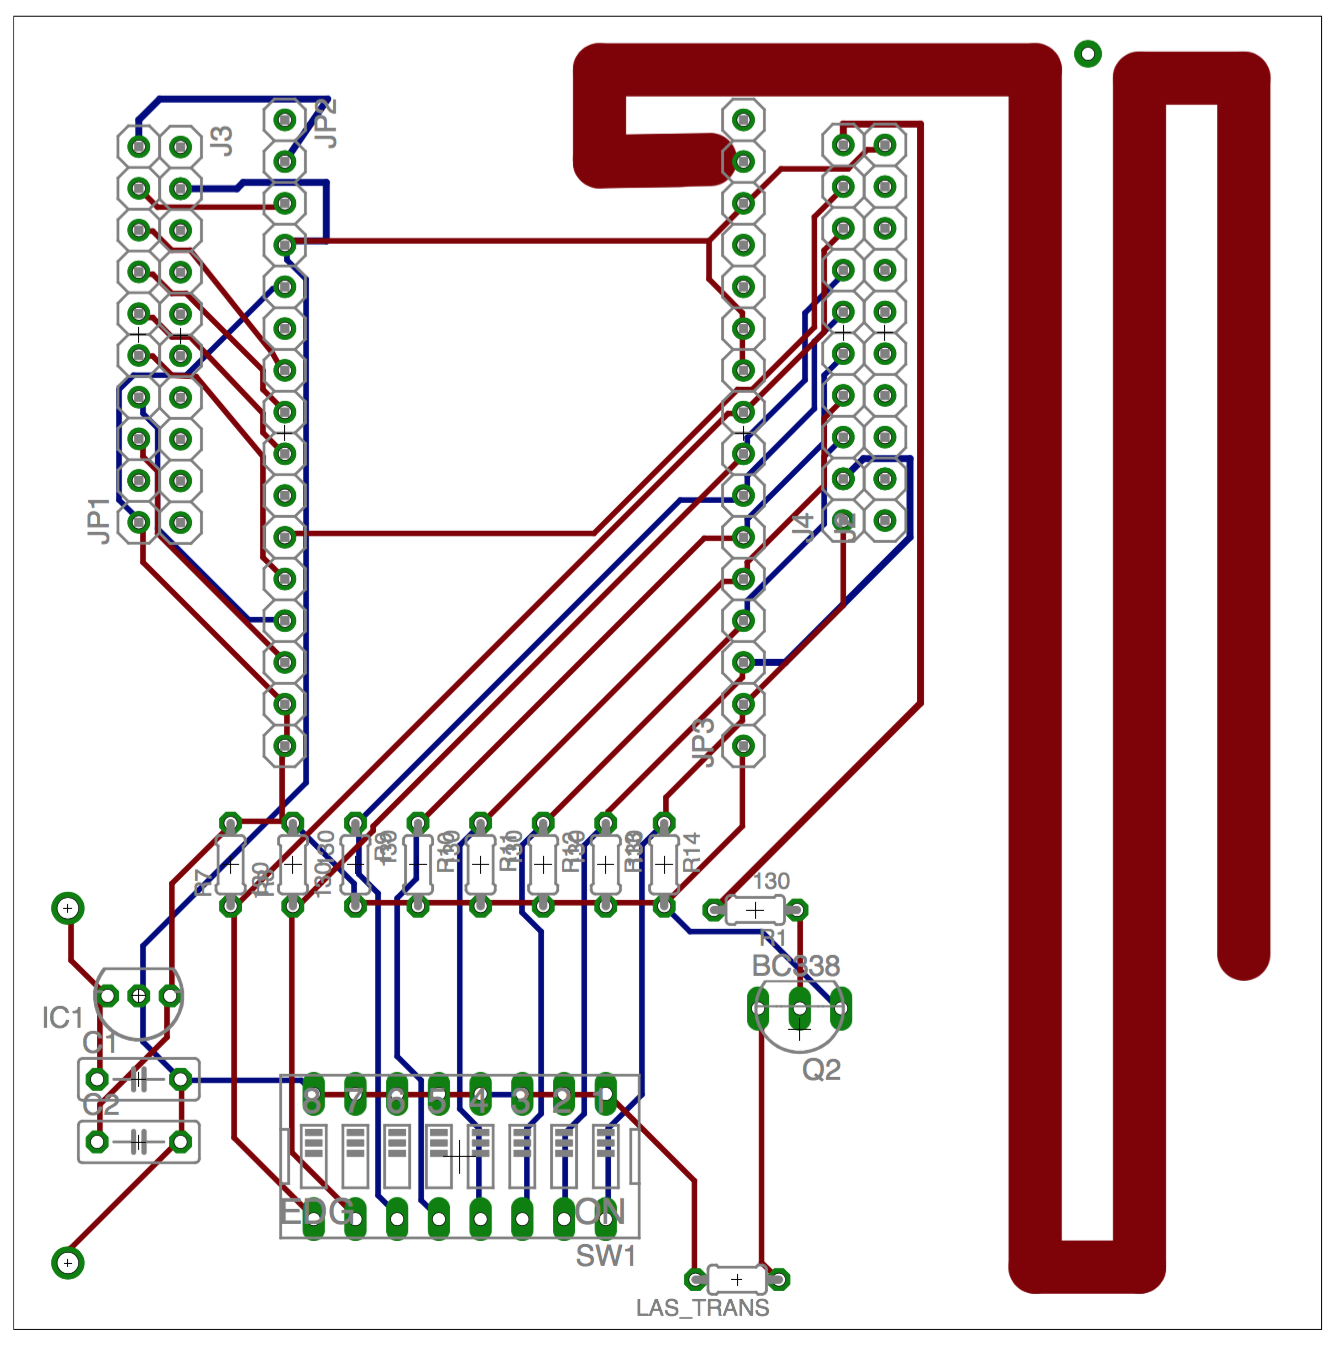
\includegraphics[scale=0.37]{interrogator_pcb.png}
	\caption{Friendly Interrogator PCB\label{fig:interrogator-pcb}}
\end{figure}

\begin{figure} [H]
	\centering
	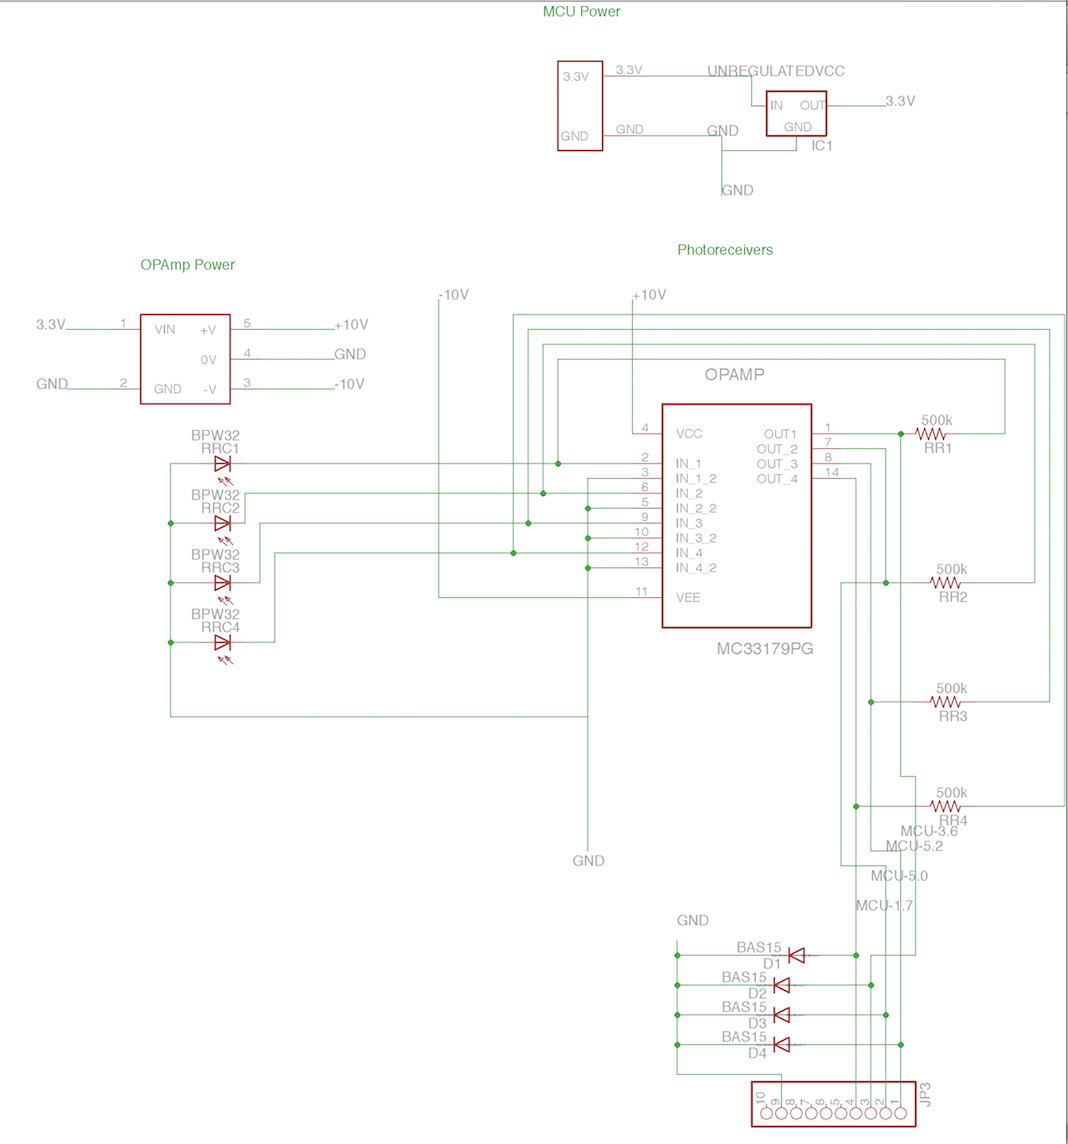
\includegraphics[scale=0.70]{target-schematic.png}
	\caption{Friendly Target Circuit Schematic \label{fig:target-schematic}}
\end{figure}

\begin{figure} [H]
	\centering
	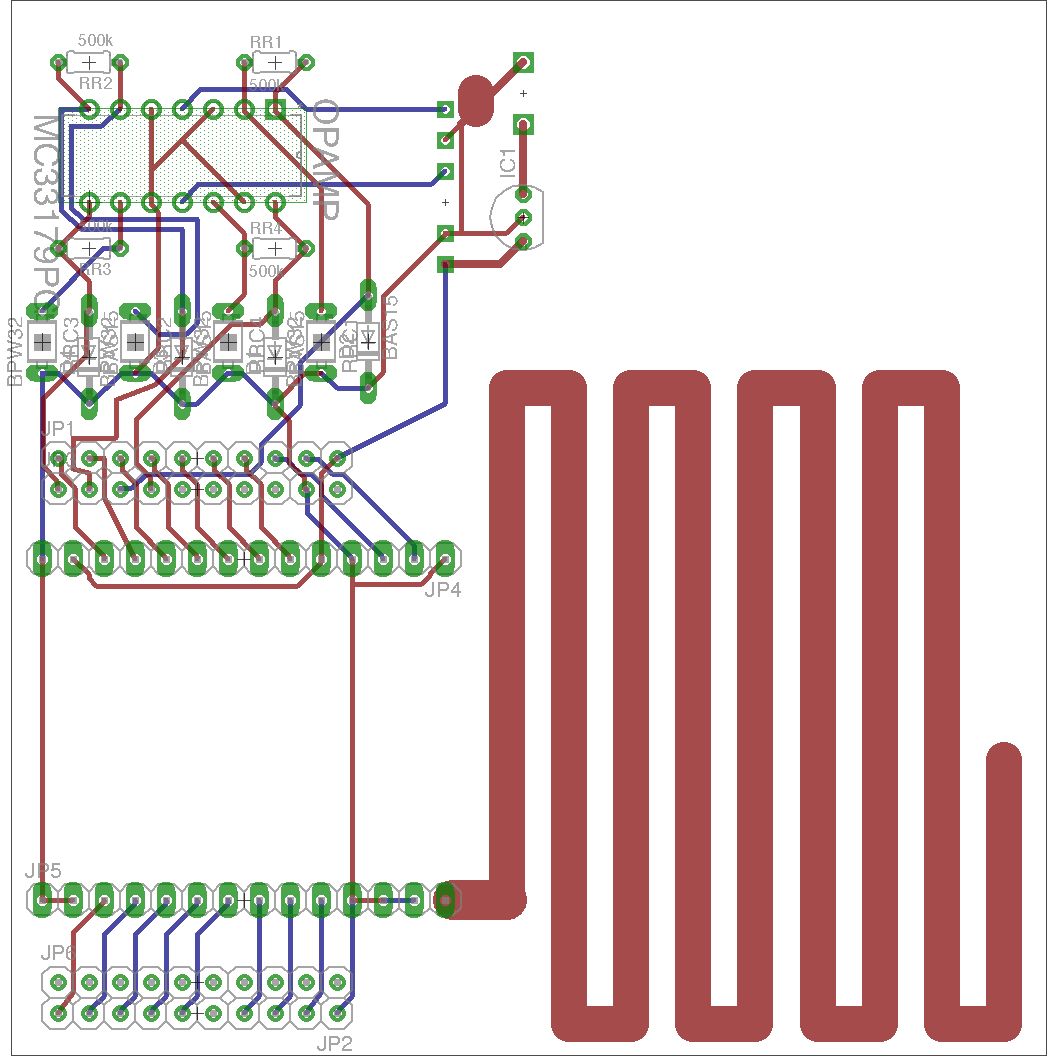
\includegraphics[scale=1.20]{target-pcb.png}
	\caption{Friendly Target PCB\label{fig:target-pcb}}
\end{figure}



\makeatletter
\def\BState{\State\hskip-\ALG@thistlm}
\makeatother

\begin{algorithm}[H]
	\caption{GetCurrentBinaryValue}\label{algo-1}
	\begin{algorithmic}[1]
		\State $\textbf{Input}: \textit{currentAnalogValue},\ \textit{lastAnalogValue},\ \textit{lastBinaryValue},\ \textit{THRESHOLD}$\\
		
		\State $\textit{dif} \gets (\textit{currentAnalogValue} - \textit{lastAnalogValue})$\\\\
		
		
		//Was a 0, now a high indicates a 1
		\If {$dif > \textit{THRESHOLD}$} \\
		\quad \Return $1$\\\\
		
		//Was a 1, now a low indicates a 0
		\ElsIf {$dif < -\textit{THRESHOLD}$} \\
		\quad \Return $0$\\\\
		
		//No change from last value
		\Else\\
		\quad \Return \textit{lastBinaryValue}
		\EndIf
	\end{algorithmic}
\end{algorithm}

\begin{algorithm}[H]
	\caption{ReceivePreamble}\label{algo-2}
	\begin{algorithmic}[1]
		\State $\textit{photoBinary} \gets \text{new}\ \textit{Array}(8)$
		\State $\textit{lastBinaryValue} \gets 0$
		\State $\textit{lastAnalogValue} \gets 0$
		\State $currentIndex \gets 0$\\
		
		\State \textbf{every} $200 \mu s$ \textbf{do}\\
		\quad // Store current value\\
		\quad $\textit{currentAnalogValue} \gets \text{analogReadPhotoreceiver}$\\
		\quad $\textit{currentBinaryValue} \gets \text{GetCurrentBinaryValue}(\textit{currentAnalogValue},$\\ 
		\hspace{7.65cm} $\textit{lastAnalogValue},$\\
		\hspace{7.65cm} $\textit{lastBinaryValue})$ \\
		\quad $\text{photoBinary}[\textit{currentIndex}] \gets \textit{currentBinaryValue}$\\
		\quad $\textit{currentIndex} = (\textit{currentIndex} + 1)\ \%\ 8$\\\\
		
		\quad // Check if last 8 received values make 10101010 
		\State \quad $\textit{lastEightValues} = \text{concat}(\text{photoBinary}[\textit{currentIndex}...8],\text{photoBinary}[0..\textit{currentIndex}])$ \\
		\quad \textbf{if} $\textit{lastEightValues} == 10101010$ \textbf{then}\\
		\quad \quad ReceivePacket\\
		
		\State \quad $\textit{lastBinaryValue} \gets \textit{currentBinaryValue}$
		\State \quad $\textit{lastAnalogValue} \gets \textit{currentAnalogValue}$
		\State \textbf{end}		
	\end{algorithmic}
\end{algorithm}

\begin{algorithm}[H]
	\caption{ReceivePacket}\label{algo-3}
	\begin{algorithmic}[1]
		\State $\textit{packet} \gets \text{new}\ \textit{Array}(8)$
		\State $\textit{lastBinaryValue} \gets 0$
		\State $\textit{lastAnalogValue} \gets 0$
		\State $currentIndex \gets 0$\\
		
		\State 8 \textbf{times}, \textbf{every} $200 \mu s$ \textbf{do}\\
		\quad // Store current value\\
		\quad $\textit{currentAnalogValue} \gets \text{analogReadPhotoreceiver}$\\
		\quad $\textit{currentBinaryValue} \gets \text{GetCurrentBinaryValue}(\textit{currentAnalogValue},$\\ 
		\hspace{7.65cm} $\textit{lastAnalogValue},$\\
		\hspace{7.65cm} $\textit{lastBinaryValue})$ \\
		\quad $\text{packet}[\textit{currentIndex}] \gets \textit{currentBinaryValue}$\\
		\quad $\textit{currentIndex}\text{++}$\\\\
		
		\State \quad $\textit{lastBinaryValue} \gets \textit{currentBinaryValue}$
		\State \quad $\textit{lastAnalogValue} \gets \textit{currentAnalogValue}$
		\State \textbf{end}\\\\
		
		\Return \textit{packet}
	\end{algorithmic}
\end{algorithm}

\begin{algorithm}[H]
	\caption{CountMissedPackets}\label{algo-4}
	\begin{algorithmic}[1]
		\State \textbf{Input}: \textit{expectedPacketValue}\\
		\State $\textit{missedPackets} \gets 0$\\
		ReceivePreambleAndPacket // Get first packet to ensure transmission started
		
		\State $100.\textbf{times}\ \textbf{do}$\\
		\quad ReceivePreambleOnce // Receive next 8 bits as preamble, ignore if not a correct preamble \\
		\quad \textbf{if} ReceivePacket $\neq$ \textit{expectedPacketValue} \textbf{then} \\
		\quad \quad \textit{missedPackets}++
		\State \textbf{end}
	\end{algorithmic}
\end{algorithm}
\clearpage

\begin{figure} [H]
	\centering
	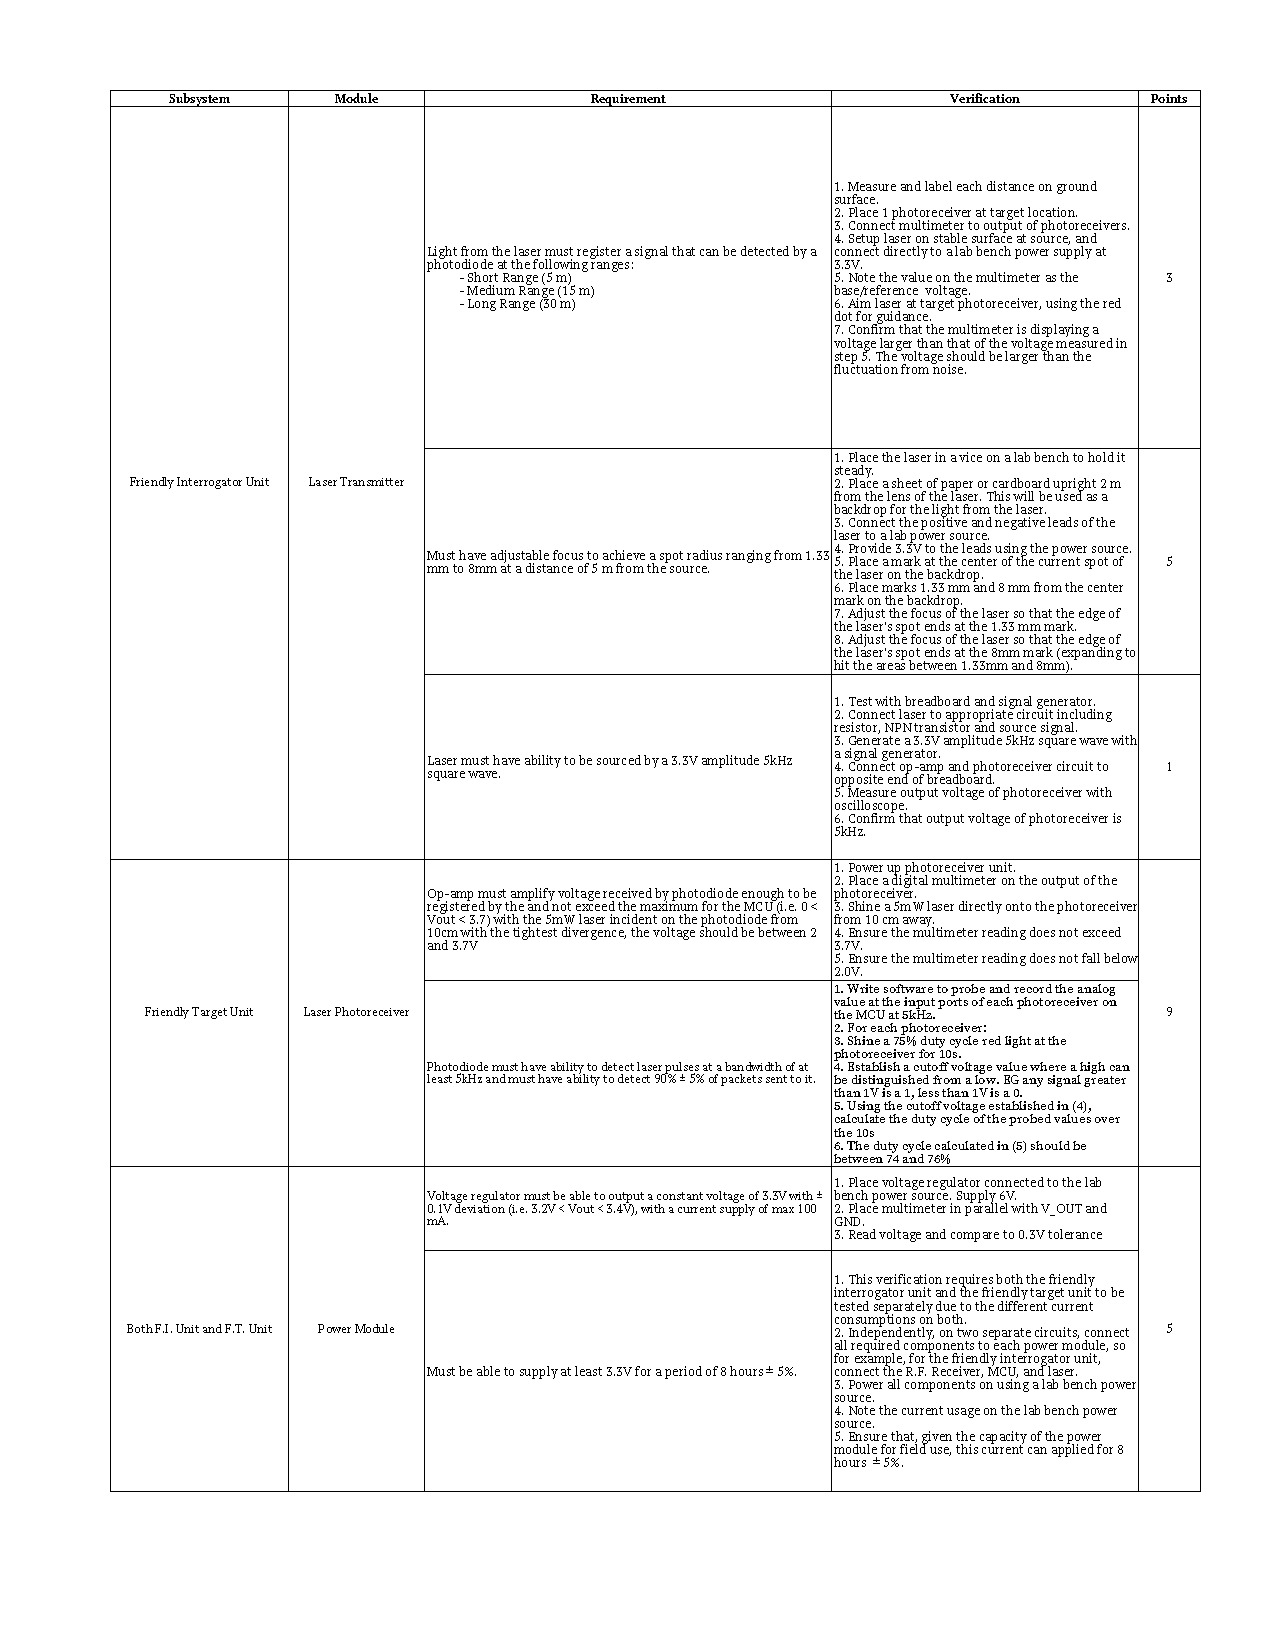
\includepdf[page=1, scale=0.85] {Requirements-Verification.pdf}
\end{figure}
\clearpage

\begin{figure} [H]
	\centering
	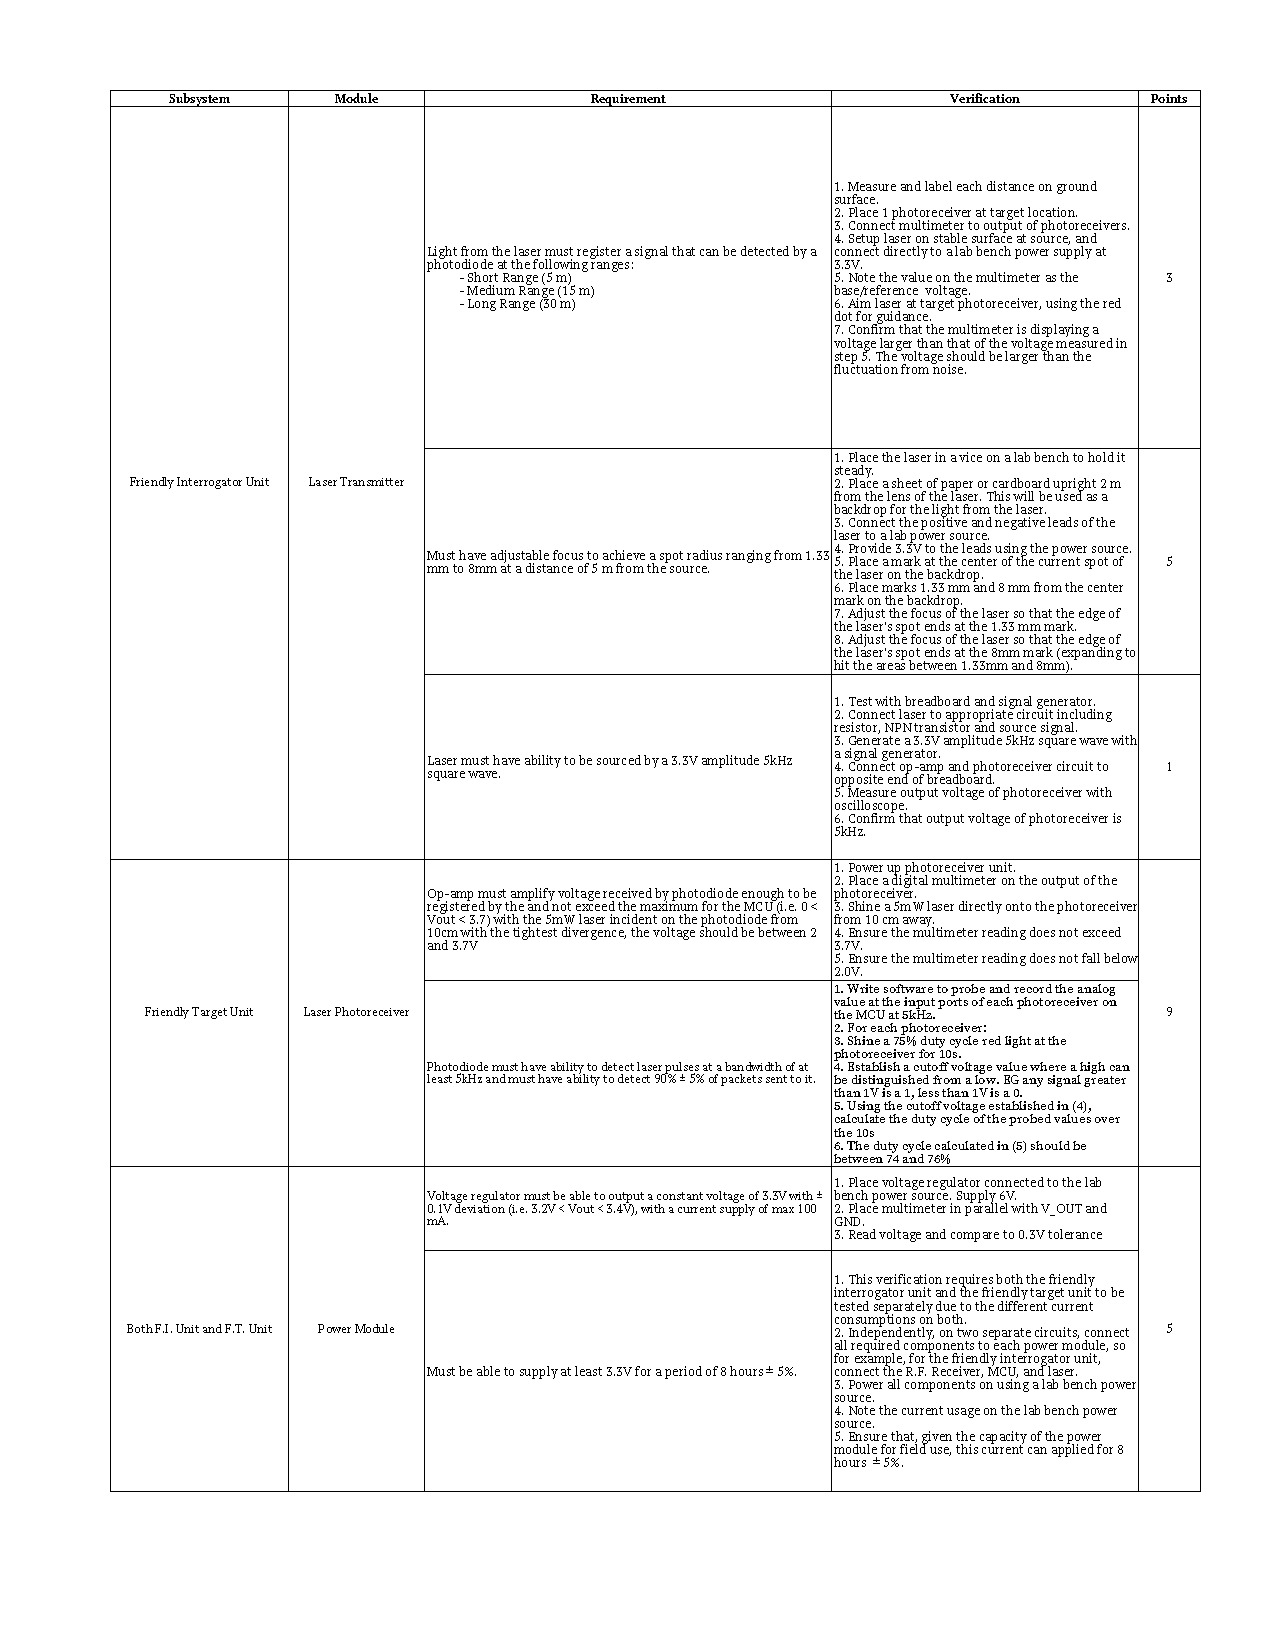
\includepdf[page=2, scale=0.85] {Requirements-Verification.pdf}
\end{figure}

\end{spacing}
\end{document}

